%! Tex program = xelatex   
\documentclass{article}
\usepackage[left=2cm, right=2cm, lines=45, top=0.8in, bottom=0.7in]{geometry}
\usepackage{xeCJK}
\usepackage{amsmath}
\usepackage{booktabs} %表格
\usepackage{graphicx}
\setmainfont{Times New Roman}
\setCJKmainfont{Songti SC}
\setCJKfamilyfont{song}{Songti SC}
\usepackage{setspace}
\setstretch{1.2} 
%-----------------------伪代码------------------
\usepackage{algorithm}  
\usepackage{algorithmicx}  
\usepackage{algpseudocode}  
\floatname{algorithm}{Algorithm}  
\renewcommand{\algorithmicrequire}{\textbf{Input:}}  
\renewcommand{\algorithmicensure}{\textbf{Output:}} 
\usepackage{lipsum}  
\makeatletter
\newenvironment{breakablealgorithm}
  {% \begin{breakablealgorithm}
  \begin{center}
     \refstepcounter{algorithm}% New algorithm
     \hrule height.8pt depth0pt \kern2pt% \@fs@pre for \@fs@ruled
     \renewcommand{\caption}[2][\relax]{% Make a new \caption
      {\raggedright\textbf{\ALG@name~\thealgorithm} ##2\par}%
      \ifx\relax##1\relax % #1 is \relax
         \addcontentsline{loa}{algorithm}{\protect\numberline{\thealgorithm}##2}%
      \else % #1 is not \relax
         \addcontentsline{loa}{algorithm}{\protect\numberline{\thealgorithm}##1}%
      \fi
      \kern2pt\hrule\kern2pt
     }
  }{% \end{breakablealgorithm}
     \kern2pt\hrule\relax% \@fs@post for \@fs@ruled
  \end{center}
  }
\makeatother
%------------------------代码-------------------
\usepackage{xcolor} 
\usepackage{listings} 
\usepackage{fontspec}
\newfontfamily\menlo{Menlo}
\setmonofont[Mapping={}]{Monaco} 
\definecolor{mygreen}{rgb}{0,0.6,0}
\definecolor{mygray}{rgb}{0.5,0.5,0.5}
\definecolor{mymauve}{rgb}{0.58,0,0.82}
\lstset{ %
backgroundcolor=\color{white},   % choose the background color
basicstyle=\footnotesize\ttfamily,        % size of fonts used for the code
columns=fullflexible,
breaklines=true,                 % automatic line breaking only at whitespace
captionpos=b,                    % sets the caption-position to bottom
tabsize=4,
commentstyle=\color{mygreen},    % comment style
escapeinside={\%*}{*)},          % if you want to add LaTeX within your code
keywordstyle=\color{blue},       % keyword style
stringstyle=\color{mymauve}\ttfamily,     % string literal style
frame=single,
rulesepcolor=\color{red!20!green!20!blue!20},
numbers=left,
 numberstyle=\tiny\menlo
% identifierstyle=\color{red},
% language=c++,
}
\begin{document}
\title{聊天程序的设计和实现}
\author{朱浩泽 1911530}
\maketitle
\section{作业说明}
\large \ \ \ \ 利用Socket,设计和编写一个聊天程序。基本要求如下:
\begin{enumerate}
  \item 设计一个两人聊天协议,要求聊天信息带有时间标签。
  \item 对聊天程序进行设计。
  \item 在Windows系统下,利用C/C++中的流式Socket对设计的程序进行实现。程序界面可以采用命令行方式,但需要给出使用方法。
  \item 对实现的程序进行测试。
  \item 撰写实验报告,并将实验报告和源码提交至本网站。
\end{enumerate}
\section{应用层协议设计}
\large
\ \ \ \ \ 本次实验传输层协议采用 TCP 协议,数据以流式传输。
\par
应用层设计的双人聊天室为客户端和服务端相互发送并接收信息,要求服务器和客户端同时在线时。客户端可以向服务器发送消息并接受服务器传来的消息,同样服务器也可以向客户端发送消息并接受客户端传输的消息。对于消息来说,每条消息具体报文\textbf{长度不能超过100个字符},并以空格或换行符表示结束,如过超过此长度,超过的部分将被自动忽略;如果一次输入中包含空格,将根据空格拆分成多个字符串分别发送。
\par
关于消息发送和接收的显示:当成功接收到消息时,将在接受到的消息前打上时间戳后显示,如“x日x时x分x秒收到消息:消息内容 ”;当成功发送消息时,将提示“消息已于x日x时x分x秒成功发送”。如果发送消息“quit()”,则证明用户即将结束聊天,则发送这条消息的端口则会显示“您已于x日x时x分x秒退出聊天室”,接收端收到该条消息后会显示“对方已于x日x时x分x秒下线退出聊天室”,至此聊天结束。
\par
聊天室将采用多线程的方式将接收消息和发送消息分开执行,用户可以随时发送并接收消息。接收到的消息按照时间顺序打印。\\
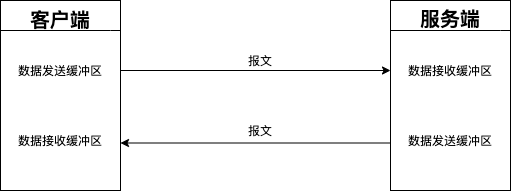
\includegraphics[scale=1.0]{1.png}
\\ 
\\ 
\section{程序设计}
\subsection{项目环境}
\large
\ \ \ \ \ 本实验在Windows10平台上使用C++11进行设计,采用visual studio 2017编译器,利用Windows自带的winsock2接口链接ws2\_32.lib库,搭建一个基础的winSock程序实现双人聊天程序的设计。
\subsection{设计思路}
\large
\paragraph{关于服务端}
服务器开启后将对客户端进行监听,当客户端上线后,将在服务端进行提醒。一旦成功连接客户端,则同时可以进行接收和发送的功能,直到收到退出的消息。
\large
\paragraph{关于客户端}
客户端开启后首先尝试连接服务器,如果服务器未开启或连接失败则直接退出程序;若服务器连接成功则同时可以进行接收和发送的功能,直到收到退出的消息。
\large
\paragraph{关于多线程}
在实际的聊天情境中,往往说话顺序并不一定是交替进行,具有不确定性。如果聊天的话语只能交替进行,则用户的使用体验将会非常不佳。所以我们对程序进行多线程设计,使发送消息和接受消息的线程分开,让用户可以随时发送消息,同时不影响消息的接收。
\newpage
\section{具体代码实现}
\subsection{服务端}
首先我们引入使用的头文件和库文件,并定义缓冲区的长度最大值为100个字符。
\begin{lstlisting}[language = c++]
#include <stdio.h>
#include <winsock2.h>
#include <iostream>
#pragma comment (lib, "ws2_32.lib")  //加载 ws2_32.dll


#define BUF_SIZE 100
\end{lstlisting}
接下来,我们创建一个WSADATA,用来存储被WSAStartup函数调用后返回的Windows Sockets数据。如果创建成功则打印“Call WSAStartup succseefully!”,创建失败便退出程序。
\begin{lstlisting}[language = c++]
WSADATA wsaData;
if (WSAStartup(MAKEWORD(2, 2), &wsaData) == 0)
{
	std::cout << "Call WSAStartup succseefully!" << std::endl;
}
else {
	std::cout << "Call WSAStartup unsuccseeful!" << std::endl;
	return 0;
}
\end{lstlisting}
然后创建套接字并对套接字进行端口绑定(使用IPV4),后进入监听状态等待客户端上线。
\begin{lstlisting}[language = c++]
//创建套接字
SOCKET servSock = socket(AF_INET, SOCK_STREAM, 0);

//绑定套接字
sockaddr_in sockAddr;
memset(&sockAddr, 0, sizeof(sockAddr));  //每个字节都用0填充
sockAddr.sin_family = PF_INET;  //使用IPv4地址
sockAddr.sin_addr.s_addr = inet_addr("127.0.0.1");  //具体的IP地址
sockAddr.sin_port = htons(1234);  //端口
bind(servSock, (SOCKADDR*)&sockAddr, sizeof(SOCKADDR));

//进入监听状态
if (listen(servSock, 20) == 0) {
	std::cout << "已进入监听状态" << std::endl;
}
else {
	std::cout << "监听状态出错" << std::endl;
	return 0;
}

//接收客户端请求
SOCKADDR clntAddr;
int nSize = sizeof(SOCKADDR);
SOCKET clntSock = accept(servSock, (SOCKADDR*)&clntAddr, &nSize);
if (clntSock > 0) {
	std::cout << "客户端上线" << std::endl;
}
\end{lstlisting}
\newpage
\noindent
在客户端上线后,调用发送和接收线程(代码在后面展示)来进行消息的发送和接收,直至程序结束关闭套接字,终止Winsock.dll的使用。
\begin{lstlisting}[language = c++]
HANDLE hThread[2];
hThread[0] = CreateThread(NULL, 0, Recv, (LPVOID)&clntSock, 0, NULL);
hThread[1] = CreateThread(NULL, 0, Send, (LPVOID)&clntSock, 0, NULL);
WaitForMultipleObjects(2, hThread, TRUE, INFINITE);
CloseHandle(hThread[0]);
CloseHandle(hThread[1]);


closesocket(clntSock);  //关闭套接字

//关闭套接字
closesocket(servSock);

//终止 DLL 的使用
WSACleanup();

return 0;
\end{lstlisting}
\subsection{客户端}
首先我们引入使用的头文件和库文件,并定义缓冲区的长度最大值为100个字符。
\begin{lstlisting}[language = c++]
#include <stdio.h>
#include <WinSock2.h>
#include <windows.h>
#include <iostream>
#include <thread>
#include <string>
#pragma comment(lib, "ws2_32.lib")  //加载 ws2_32.dll

#define BUF_SIZE 100
\end{lstlisting}
接下来,我们创建一个WSADATA,用来存储被WSAStartup函数调用后返回的Windows Sockets数据。如果创建成功则打印“Call WSAStartup succseefully!”,创建失败便退出程序。
\begin{lstlisting}[language = c++]
WSADATA wsaData;
if (WSAStartup(MAKEWORD(2, 2), &wsaData) == 0)
{
	std::cout << "Call WSAStartup succseefully!" << std::endl;
}
else {
	std::cout << "Call WSAStartup unsuccseeful!" << std::endl;
	return 0;
}
\end{lstlisting}
然后创建套接字并对套接字进行端口绑定(使用IPV4),对服务端进行连接。若服务端未开启,则显示“聊天室未上线”并退出程序。
\begin{lstlisting}[language = c++]
sockaddr_in sockAddr;
memset(&sockAddr, 0, sizeof(sockAddr));  //每个字节都用0填充
sockAddr.sin_family = PF_INET;
sockAddr.sin_addr.s_addr = inet_addr("127.0.0.1");
sockAddr.sin_port = htons(1234);
SOCKET sock = socket(AF_INET, SOCK_STREAM, 0);
if (connect(sock, (SOCKADDR*)&sockAddr, sizeof(SOCKADDR)) == 0)
{
	std::cout << "成功进入聊天室" << std::endl;
}
else {
	std::cout << "聊天室未上线" << std::endl;
	return 0;
}
\end{lstlisting}
在连接到客户端后,调用发送和接收线程(代码在后面展示)来进行消息的发送和接收,直至程序结束关闭套接字,终止Winsock.dll的使用。
\begin{lstlisting}[language = c++]
HANDLE hThread[2];
hThread[0] = CreateThread(NULL, 0, Recv, (LPVOID)&sock, 0, NULL);
hThread[1] = CreateThread(NULL, 0, Send, (LPVOID)&sock, 0, NULL);
WaitForMultipleObjects(2, hThread, TRUE, INFINITE);
CloseHandle(hThread[0]);
CloseHandle(hThread[1]);
closesocket(sock); 
WSACleanup(); 
return 0;
\end{lstlisting}
\subsection{消息接收与发送线程}
发送线程
\begin{lstlisting}[language = c++]
DWORD WINAPI Send(LPVOID sockpara) {
	SOCKET * sock = (SOCKET*)sockpara;
	char bufSend[BUF_SIZE] = { 0 };
	while (1) {
		//printf("Input a string: ");
		std::cin >> bufSend;
		int t = send(*sock, bufSend, strlen(bufSend), 0);
		if (strcmp(bufSend, "quit()") == 0)
		{
			SYSTEMTIME st = { 0 };
			GetLocalTime(&st);
			closesocket(*sock);
			std::cout << "您已于" << st.wDay << "日" << st.wHour << "时" << st.wMinute << "分" << st.wSecond << "秒退出聊天室" << std::endl;
			return 0L;
		}
		if (t > 0) {
			SYSTEMTIME st = { 0 };
			GetLocalTime(&st);
			std::cout << "消息已于" << st.wDay << "日" << st.wHour << "时" << st.wMinute << "分" << st.wSecond << "秒成功发送\n" ;
			std::cout << "-------------------------------------------------------------" << std::endl;
		}
		memset(bufSend, 0, BUF_SIZE);  
	}
}
\end{lstlisting}
接收线程
\begin{lstlisting}[language = c++]
DWORD WINAPI Recv(LPVOID sock_) {
	char bufRecv[BUF_SIZE] = { 0 };
	SOCKET *sock = (SOCKET*)sock_;
	while (1) {
		int t = recv(*sock, bufRecv, BUF_SIZE, 0);
		if (strcmp(bufRecv, "quit()") == 0)
		{
			SYSTEMTIME st = { 0 };
			GetLocalTime(&st);
			closesocket(*sock);
			std::cout << "对方已于" << st.wDay << "日" << st.wHour << "时" << st.wMinute << "分" << st.wSecond << "秒下线退出聊天室" << std::endl;
			return 0L;
		}
		if (t > 0) {
			SYSTEMTIME st = { 0 };
			GetLocalTime(&st);
			std::cout << st.wDay << "日" << st.wHour << "时" << st.wMinute << "分" << st.wSecond << "秒收到消息:";
			printf(" %s\n", bufRecv);
			std::cout << "-------------------------------------------------------------" << std::endl;
		}
		memset(bufRecv, 0, BUF_SIZE);
	}
}
\end{lstlisting}
\section{实验中遇到的问题与思考}
在实验最初实现多线程时,对每个线程的传入参数为sockAddr,并在每个线程的循环的每次迭代中创建套接字,在迭代的末尾关闭套接字,其代码大致如下:\\
\begin{lstlisting}[language = c++, title = 最初的错误代码]
//调用线程的语句
hThread[1] = CreateThread(NULL, 0, Send, (LPVOID)&sockAddr, 0, NULL);
//线程函数如下
DWORD WINAPI Recv(LPVOID sock_) {
	sockaddr_in *sockAddr = (SOCKET*)sock_;
    char bufRecv[BUF_SIZE] = {0};
    while(1){
        //创建套接字
        SOCKET sock = socket(PF_INET, SOCK_STREAM, IPPROTO_TCP);
        connect(sock, (SOCKADDR*)&(*sockAddr), sizeof(SOCKADDR));
        //获取用户输入的字符串并发送给服务器

        recv(sock, bufRecv, BUF_SIZE, 0);
        //输出接收到的数据
        printf("Message form server: %s\n", bufRecv);
        memset(bufRecv, 0, BUF_SIZE);  //重置缓冲区
        closesocket(sock);  //关闭套接字
    }
}
\end{lstlisting}
如果按照这种方式执行代码,程序会一直陷入发送消息或接收消息的线程中。如果陷入的是接收线程,则接收不到任何消息,但程序一直在进行迭代;如果陷入的是发送线程,程序依旧在无限迭代,但输入的内容对方无法接收。后进行更改,将sock在主程序中进行初始化,并以普通方式传入两个线程中,问题依然得不到解决。最终,在将传入参数改为在主函数中创建的socket的引用后,程序可以按照设计理念运行,问题得到解决。通过查阅资料和动手实验发现,在实验中,我们采用的多线程方式,如果socket在线程的循环体中创建,或者只是简单的传socket进入函数(相当于在栈中创建了两个新的套接字),则会在并行执行的时候发生两个socket同时请求一个端口的问题(没有设置copy机制)而导致错误。但如果采用引用的方式,传入的是套接字的地址,则两个线程共用一个套接字,在发送消息和接收消息时进行复用,便能够消除上述的问题。经过测试,上述问题还可以通过设置Recv、Send为阻塞模式或设置端口的copy机制进行解决。
\section{程序使用演示}
程序在使用时应当先开启服务端,再开启客户端。否则客户端无法连接到服务端,将会自动退出程序。启动成功截图如下:\\
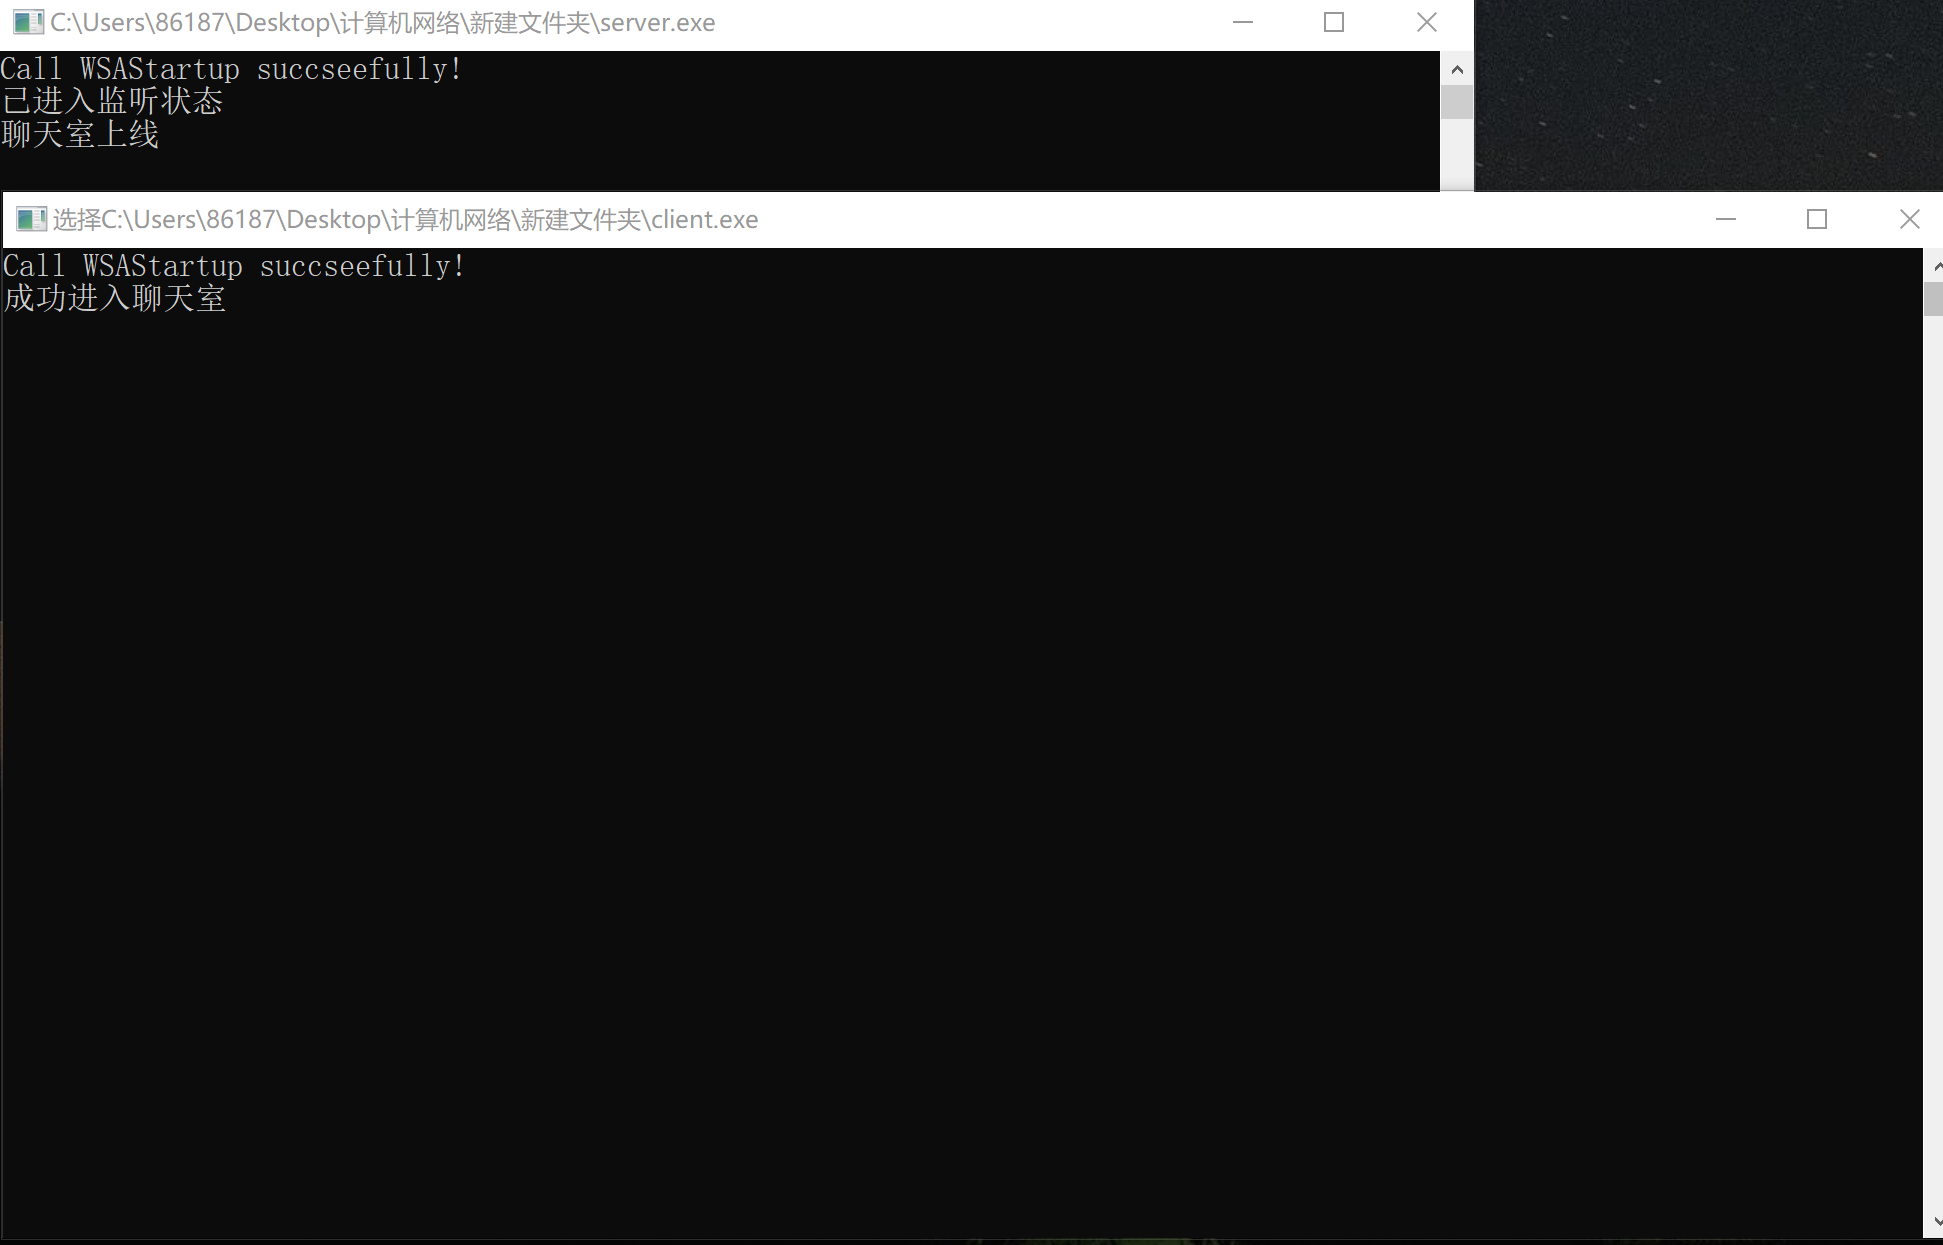
\includegraphics[scale=0.4]{2.png}\\
\newpage
\noindent 聊天截图展示如下:\\
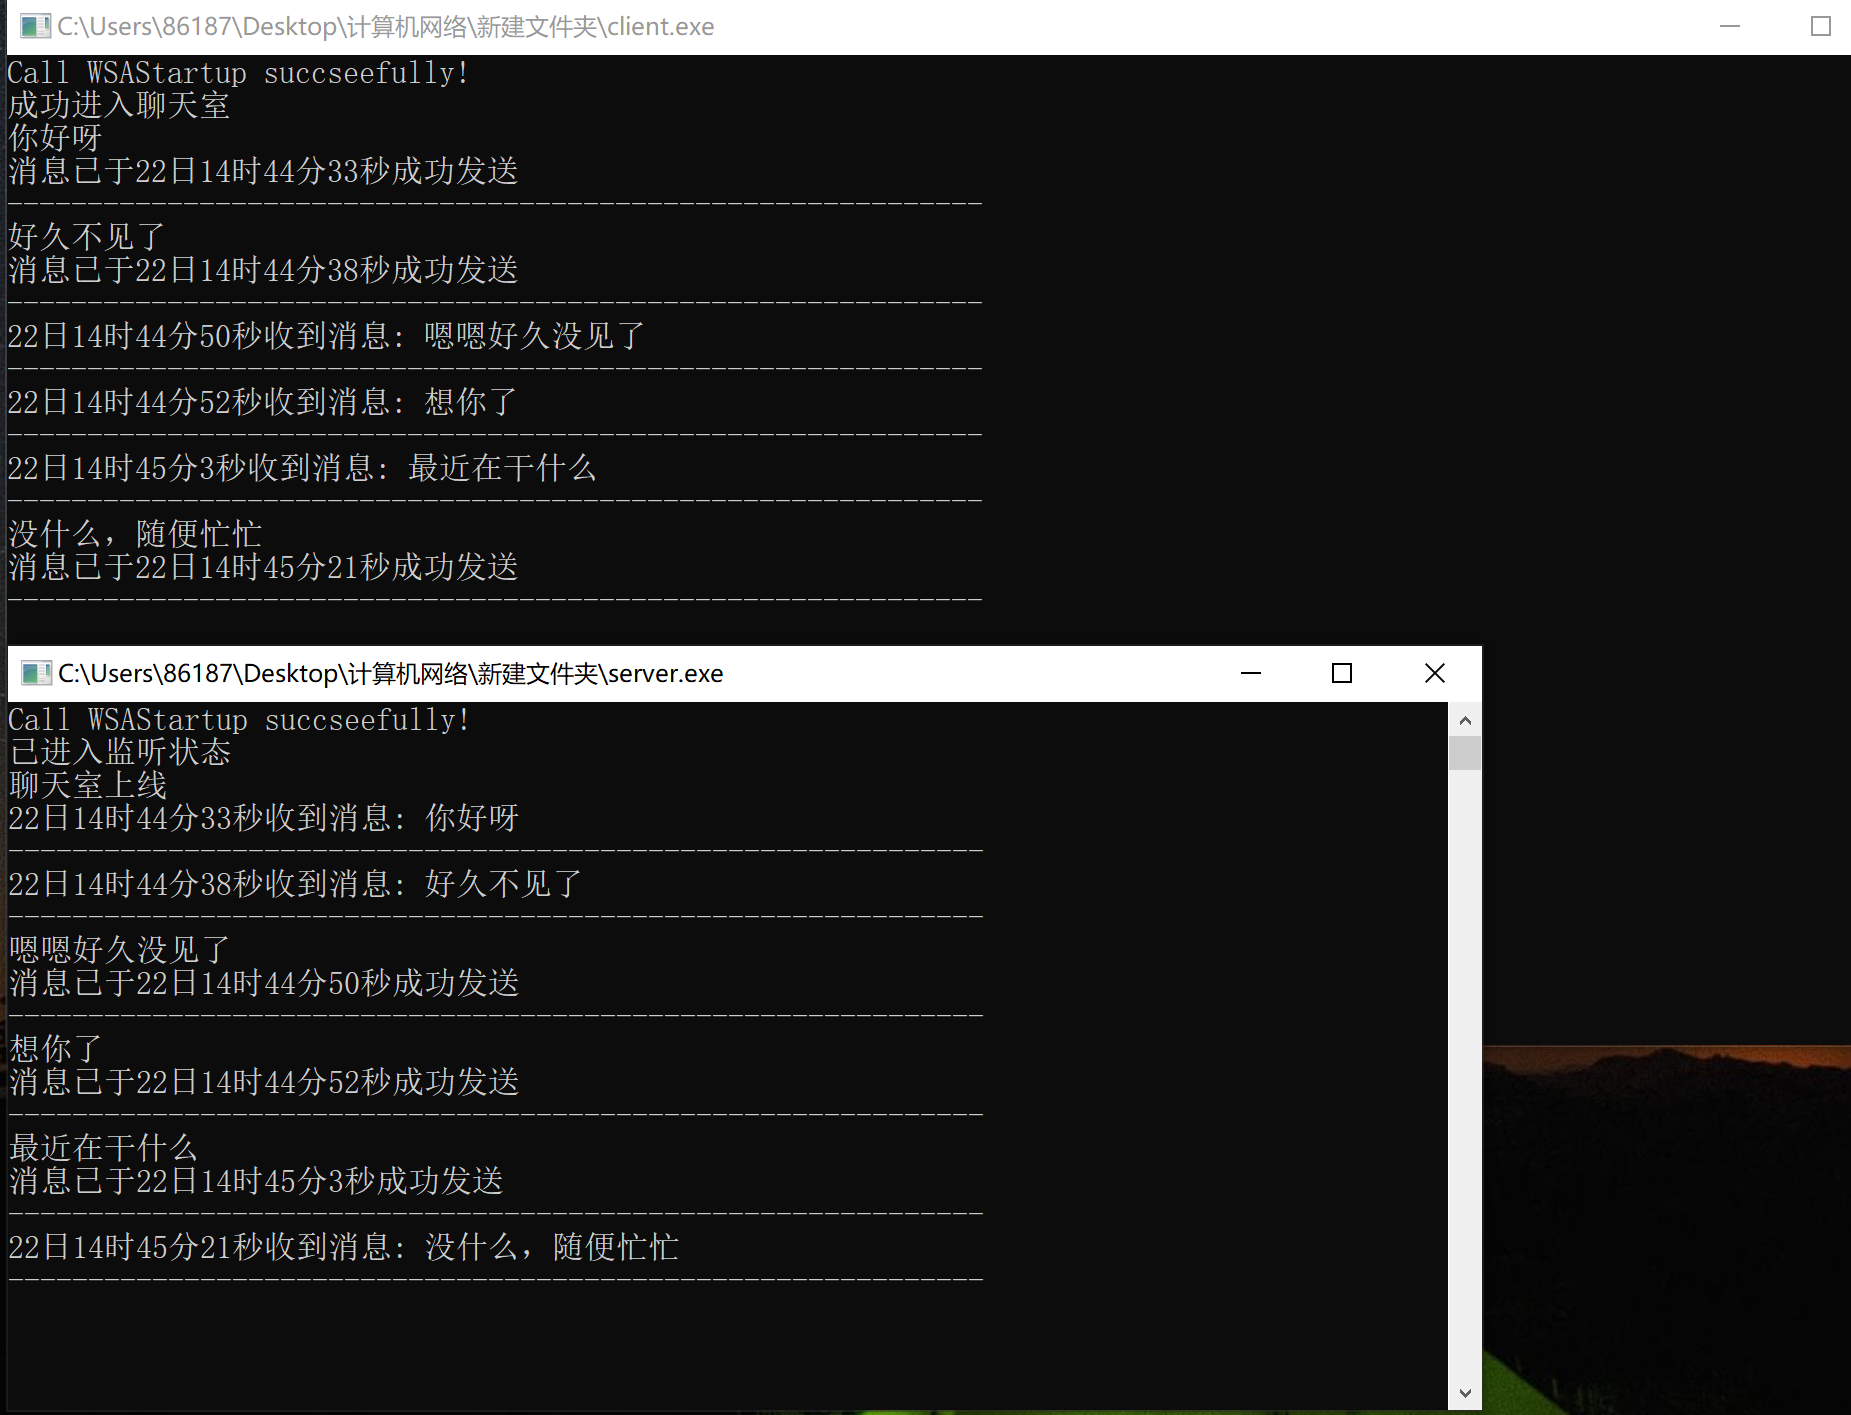
\includegraphics[scale=0.4]{3.png}\\
\\ 
输入“quit()”结束聊天,截图如下:\\
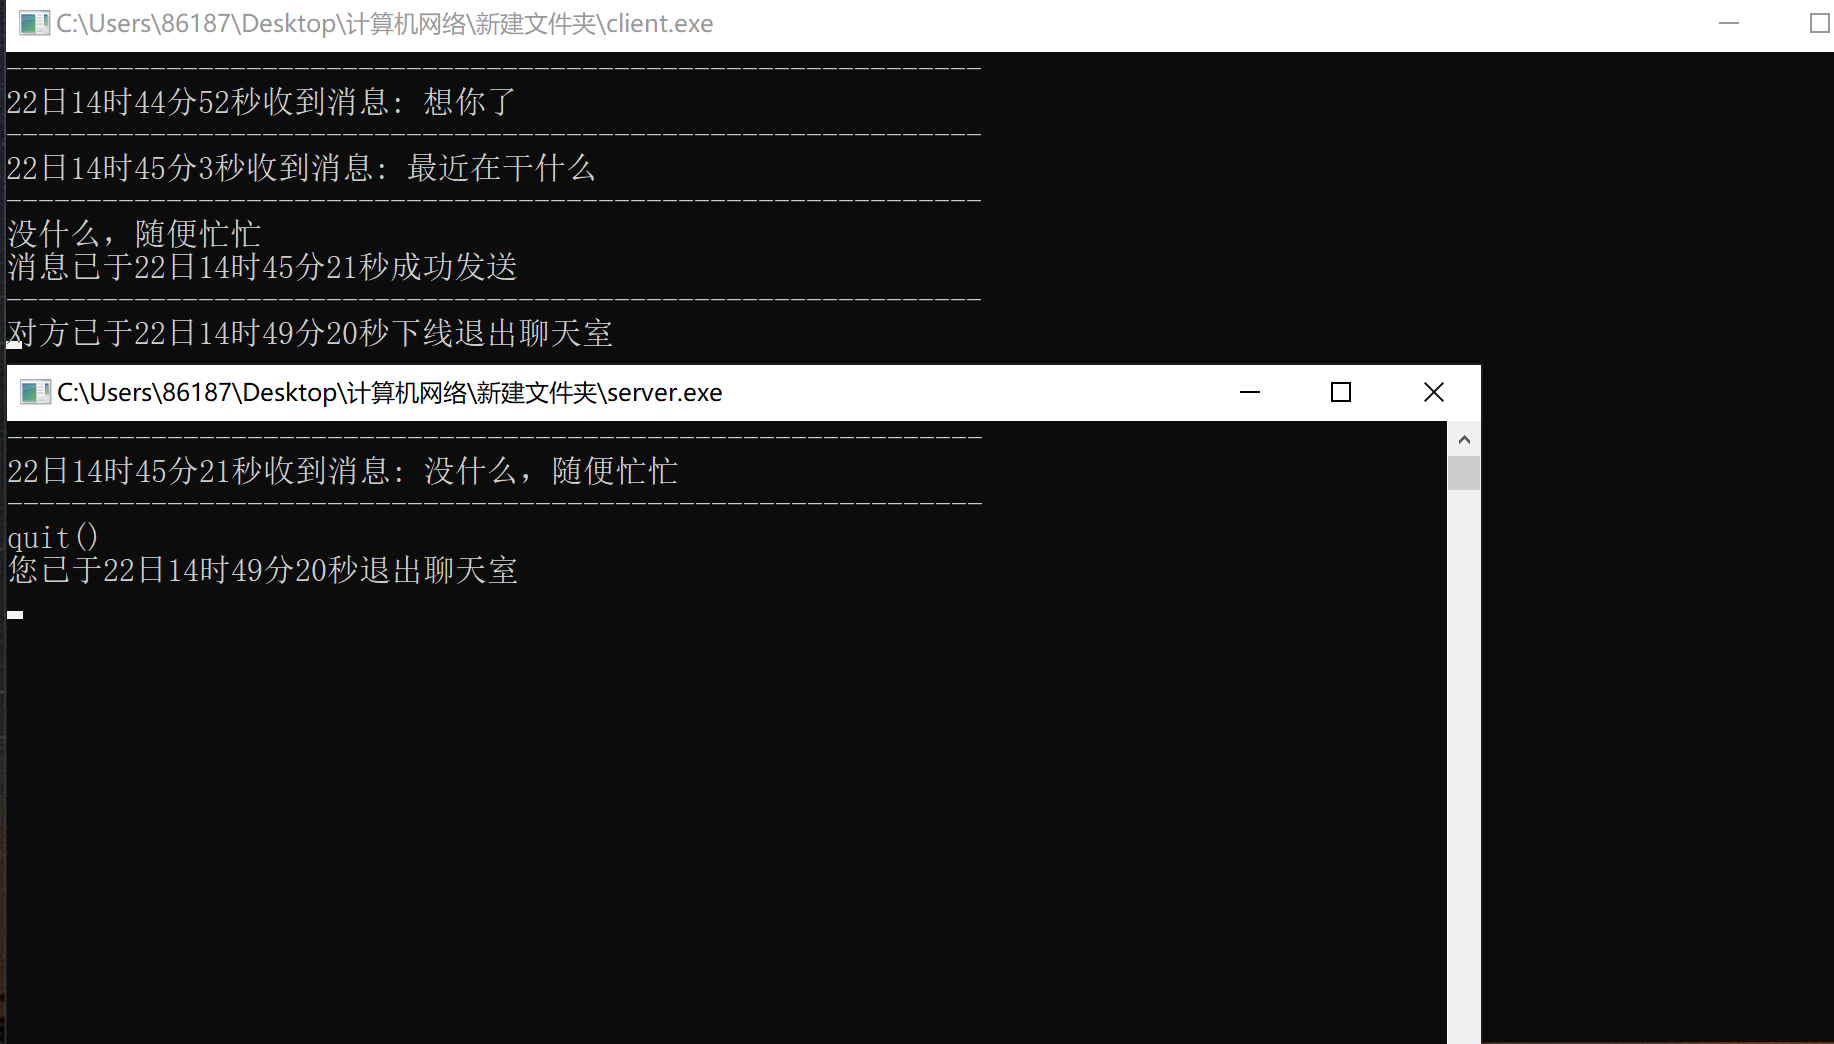
\includegraphics[scale=0.4]{4.png}
\end{document}
